\section{What is Entanglement and what is it telling us about the spacetime? \checkmark}
\FloatBarrier	
	\begin{figure}[tbp]
		\begin{center}
			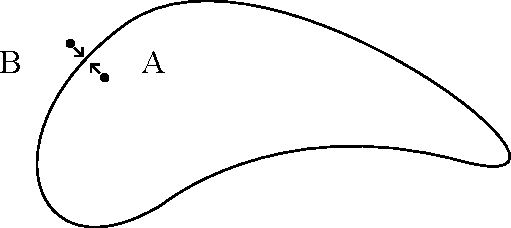
\includegraphics[scale=1]{entangledcorr}
			\caption{This is a decomposed Hilbert space into regions $A$ and $B$ by their tensor product of their fields. The to dots symbolise the two-point functions which are diverging while aproaching each other (the arrows). The boundary between these two regions is called the \textit{entangling surface}.} \label{entangling_surface}
		\end{center}
	\end{figure}		
	In relativistic QFT, the ground state has correlations between field operators at spatially separated points. Here we can use \textit{entanglement} as an explanation.
	
	But at first, let's start from the beginning:
	\\
	We have $\rho$ which is a quantum state on Hilbert space $\Hil$ and is called \textit{density matrix}. Quantum states are illustrated in operators, here: $\rho$ is a non-negative hermitian operator of trace 1. If it can be written in the form\footnote{Here $|\psi\rangle$ is some element of $\Hil$ with norm 1.}
		\begin{equation}
			\rho=|\psi\rangle \langle\psi|,
		\end{equation}
	 the quantum state is called \textit{pure}. If a state is not pure, it is \textit{mixed}.
	 
	 While doing an experiment, we will a measure an outcome $i$, which is always related to a projection operator $\Pi_i$ with a probability of measuring $i$, that looks like: 
		 \begin{equation}
	 		P(i)=\mathrm{tr}(\rho\Pi_i).
	 	\end{equation}
	 For finding out, whether a given state $\rho$ is pure or mixed, we define a function $S$ for convenience:
		\begin{equation}
			S(\rho)\equiv -\mathrm{tr}(\rho \log \rho)
		\end{equation}	 	
	And $S(\rho)$ is called the \textit{Von Neumann Entropy} or \textit{information entropy}. 
	Its proberties are:
	\FloatBarrier
	\begin{itemize}
		\item[•] for any unitary operator $U$: $S(U^\dagger \rho U)=S(\rho)$
		\item[•] $S(\rho)\geq 0$, with equality if and only if $\rho$ is pure. 
		\item[•] for $d$ is the dimension of $\Hil$: $S(\rho)\leq \log d$, with equality if and only if $\rho$ is maximally mixed.
		\item[•] The entropy of the average over a set of states is at least equal to the average of all their individual entropies. This is also called \textit{concavity} and is defined as:
		\begin{equation}
			S \left(\sum_i \lambda_i \rho_i \right) \geq \sum_i \lambda_i S(\rho_i),
		\end{equation}
			while $\lambda_i$ is any set of non-negative numbers with $\sum_i \lambda_i =1$.
	\end{itemize}
	\FloatBarrier
	Now, let's have a look at an entangled state written in the two-qubit state:
		\begin{equation}
			|\Psi\rangle = \frac{1}{\sqrt{2}} \left(\ket{00} + \ket{11} \right)
		\end{equation}
	Here, the full state is pure, but the reduced state on either qubit ($\ket{00}$ or $\ket{11}$) is mixed. \\
	
	Just a short explanation what 'qubits' are: \\
	It is the spin $1/2$-particle system with a standard basis $\{\ket{0}, \ket{1}\}$. So the particles can just have spin 'up' or 'down'. A ket in the form $\ket{00}$ for example, the first particle has spin up in one region, the second spin up in an other region.
	\\ \\	
	In \textbf{Figure \ref{entangling_surface}} the Hilbert space was decomposed into a tensor product of the degrees of freedom in a region $A$ and the its complement $B$. From the end of chapter \ref{QFT} we know that the correlation functions are divergent at short distances which means that, if the two points at the boundary between $A$ and $B$, the correlation becomes infinite. But what does that mean in respect to entanglement? Well, in the ground state there must be an infinite amount of entanglement between neighboring regions. 
	
	
	Another way of illustrating entanglement in QFT is the Reeh-Schlieder theorem \footnote{If you are interested in the detail \cite{StreaterWightman}}. This says, that while acting on the vacuum $\ket{\Omega}$ with operators of any region $A$, a set of states which is dense in full Hilbert space can be produced. This means if a local operator acts on the vacuum for example in your bedroom, we can create the moon. This is possible because of the highly entangled nature of the vacuum. \marginpar{Soll ich das wirklich reinschreiben?} 
	
%	Bipartite systems are the ones whose Hilbert space can be written as a tensor product\footnote{Watch out! The tensor product $\otimes$ is not the direct sum $\oplus$.}:
%	 	\begin{equation}
%	 		\Hil=\Hil_A \otimes \Hil_B
%	 	\end{equation}
%	 In quantum mechanics they describe the composition of two independent physical systems and can be \textit{entangled}, which means, that the reduced density matrices $\rho_A$ and $\rho_B$ can be mixed even if the joint state $\rho_{AB}$ is pure.
%	 
	
\FloatBarrier